\section{Hidden comunication by targeted reflections}

We will start from the paper \textit{Reconfigurable Intelligent Surface: Reflection Design Against Passive Eavesdropping} \cite{9328149}, explaining how to hide communication between two actors from eavesdroppers using Reconfigurable Intelligent Surfaces, then expanding it to multiple receiving users at the same time.

\subsection{The paper problem mathematics}

\begin{figure}[H]
  \centering
  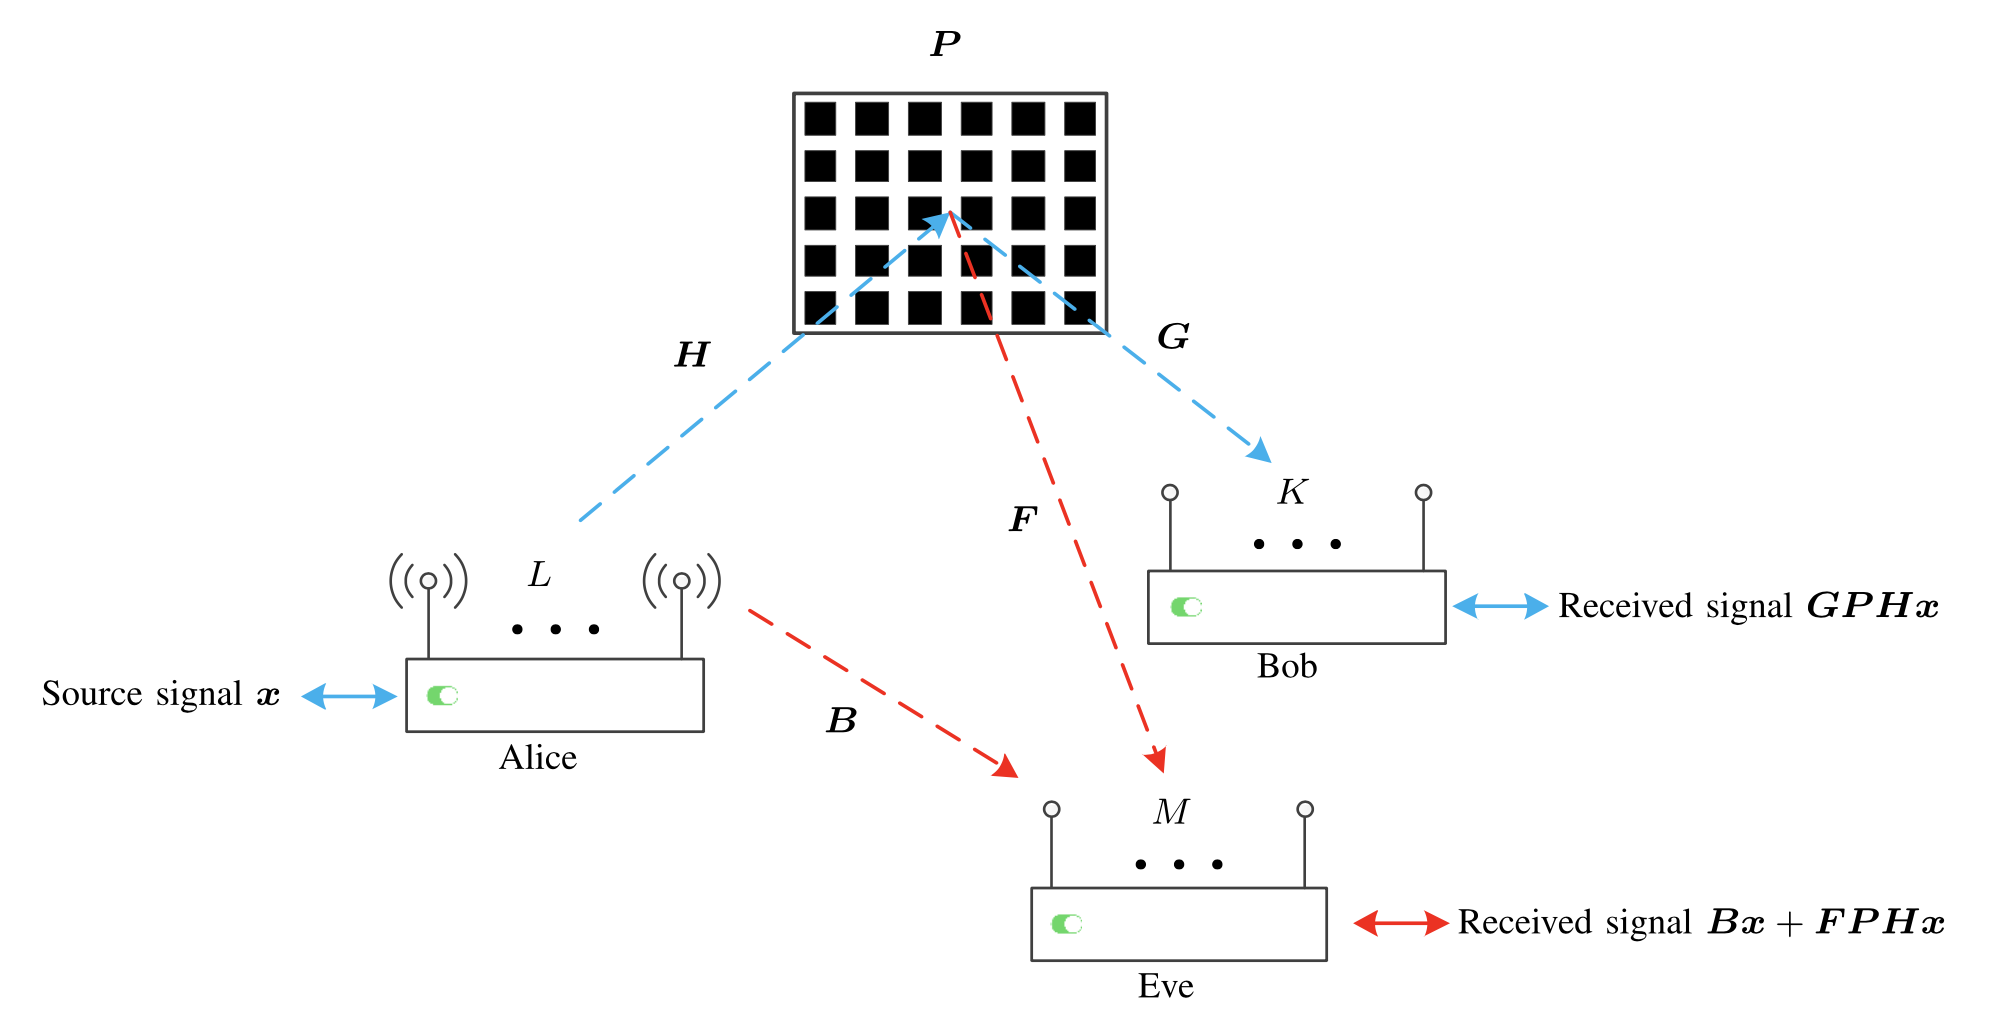
\includegraphics[width=\linewidth]{imgs/problem-description.png}
  \caption{Setup}
  \label{fig:correlation_sk}
\end{figure}

In \cite{9328149}, the authors studied how to use RISs to allow communications between two users without LOS, while making the signal undeciphrable for eavesdroppers. We call $L$ the transmitter's antennas, $K$ the receiver's antennas, $M$ the eavesdropper's antenna, and $N$ the RIS reflecting elements. We assume $L \ge K \ge 2$.

We define $H \in \C^{NxL}$ the channel response from the transmitter to the RIS, $G \in \C^{KxN}$ the channel response from the RIS to the receiver, $P = diag\{p\} \in \C^{NxN}$ a diagonal matrix in which the $n$th diagonal element represents the reflection coefficient of the $n$th unit at the RIS.

The objective is making the receiver's final signal $GPH$ a diagonal matrix, while making every possible eavesdropper's final signal a full matrix.

We will leave for now the technical details of why this would achieve secrecy for the legitimate users to the original paper, and will just focus on the mathematics behind the calculation. Our final objective will be to generalize these calculations to $J$ receving users and multiple RISs used in parallel and in sequence.

Formally, the condition we want to satisfy is:

\begin{equation}
  || [GPH]_{:,1:K} - [[GPH]_{:,1:K}]_{diag} || ^2 = 0
\end{equation}

Where $[GPH]_{:,1:K} \in \C^{KxK}$ denotes the first K columns of the matrix $GPH \in \C^{KxL}$.

Given

\begin{equation}
  W = \sum_{i,j = 1, i \ne j}^{K} (g_{j,:} \odot h_i^T)^H (g_{j,:} \odot h_i^T)
\end{equation}

The formula (1) can be rewritten as

\begin{equation}
  Wp = 0
\end{equation}

and the solutions of $p$ can be found in the null space of $W$. Using singular value decomposition (SVD), we can decompose

\begin{equation}
  W = R \lambda V^H
\end{equation}

Taken $U \in \C ^ {Nx(N-(K^2 - K))}$ the last $N-(K^2 - K)$ columns of the left singular matrix $R$. We then have

\begin{equation} p = Uq \end{equation}

and

\begin{equation}WU = 0\end{equation}

[TODO: EXPLANATION AND CITATION NEEDED], so all together we have

\begin{equation}
  WUq = 0
\end{equation}

being true, and $q \in \C^{N-(K^2 - K)}$ can be a random vector.

\subsection{Expanding to multiple users}

In real life scenarios, we deal with more than two communicating actors. We want to expand the findings of this paper by having it support multiple RISs in series and multiple receivers from the same transmitter. Once we have those, we can generalize it to also have receivers getting signals from multiple indipendent reflections of RISs.

We will first, however, make some semplifications about the actors by having $L = K$ for all of them. We will still consider one transmitter, with $J \ge 1$ receivers.

\subsubsection{Reflecting to multiple users}

We consider the case where the transmitter wants to send the signal to $J$ receivers without LOS. The condition we want to satisfy is

\begin{equation}
  \forall j \in [1...J] \rightarrow || G_jPH - [G_jPH]_{diag} || ^2 = 0
\end{equation}

\begin{equation}
  \forall j \in [1...J] \rightarrow W_jp = 0
\end{equation}

\begin{equation}
  \begin{bmatrix}
    W_1  \\
    W_ 2 \\
    ...  \\\
    W_j
  \end{bmatrix}
  p = 0
\end{equation}

\begin{equation}
  \begin{bmatrix}
    W_1  \\
    W_ 2 \\
    ...  \\\
    W_j
  \end{bmatrix}
  = W \in \C ^ {JNxN}, W = R \lambda V^H
\end{equation}

The problem we have now is that $W$ is not a square matrix anymore, so we cannot use the last $N - (K^2 - K)$ columns of $R$ to calculate the null space and $p$ with its linear combination.

We can, however, use the the last $N - (K^2 - K)$ rows of $V^H$, then apply again the hermitian transposition (transpose, then apply the complex conjugation) [TODO: EXPLANATION AND CITATION NEEDED].

Take $U_1 \in \C ^ {N - J(K^2 - K) x N}$ the last $N - (K^2 - K)$ rows of $V^H$, and
\begin{equation}
  U = U_1^H \in \C ^ {N x N - J(K^2 - K)}
\end{equation}

We now can apply the same method as before

\begin{equation}p = Uq\end{equation}

\begin{equation}WU = 0\end{equation}

\begin{equation}WUq = 0\end{equation}

\subsubsection{RISs in parallel}

Given the previous property, it follows that we can use $M$ multiple RIS, each one reflecting the signal to $J$ multiple receivers. For the receiver $j \in [1, J]$, we have

\begin{equation}
  \sum_{m=1}^M G_j P_m H_m x = (\sum_{m=1}^M G_j P_m H_m) x =
\end{equation}

The sum of diagonal matrixes is still a diagonal matrix, so the property still holds.

\subsubsection{RISs in series}

We consider the case where the signal is bounced between $M$ RISs in this way:

\begin{equation}
  \text{Transmitter} \rightarrow \text{RIS 1} \rightarrow ... \rightarrow \text{RIS M} \rightarrow \text{Receiver}
\end{equation}

\begin{equation}
  || GP_1...P_MH - [GP_1...P_MH]_{diag} || ^2 = 0
\end{equation}

Since $P_i = diag\{p_i\}$, we can rewritten

\begin{equation}
  P_1...P_M = diag\{p_1\}...diag\{p_M\} = diag\{p_1 \odot ... \odot p_M\}
\end{equation}

So we can write

\begin{equation}
  P = diag\{p_1 \odot ... \odot p_M\}, p = p_1 \odot ... \odot p_M
\end{equation}

Once we find $p$ using the same way as before, we can now decompose it so that

\begin{equation}
  p[i] = p_1[i] * ... * p_M[i]
\end{equation}

We can generate $p_1, ..., p_{M-1}$ as random reflections, and calculate the last one based on the previous. An advantage we get is that eavesdroppers listening from a middle RIS will not be able to decipher the signal either. Given $r_i \in [0, 1]$ the absorption coefficient, and $\theta_i \in [0, 2\pi]$ the phase shift, we can choose them randomly for all RIS $p_m$ vectors, but the last one.

\begin{equation}
  \forall m \in [1, M-1] : p_m[i] = \eta * r_i * e^{j\theta_i}
\end{equation}

\begin{equation}
  p_M[i] = p[i] / (p_1[i] * ... * p_{M-1}[i])
\end{equation}
